
%(BEGIN_QUESTION)
% Copyright 2006, Tony R. Kuphaldt, released under the Creative Commons Attribution License (v 1.0)
% This means you may do almost anything with this work of mine, so long as you give me proper credit

Skisser kurvene for regulatorutgang og prosessvariabel for to scenarier: ett hvor prosessen er {\it integrerende}, og det andre hvor det er {\it dødtid} i prosessmålingen. I begge tilfeller, anta at regulatoren er satt i manuell modus og gitt en liten sprangendring. Skissene dine skal vise denne sprangendringen sammen med prosessvariabelens respons:

\vskip 10pt

\noindent
{\bf Integrerende prosess:}

$$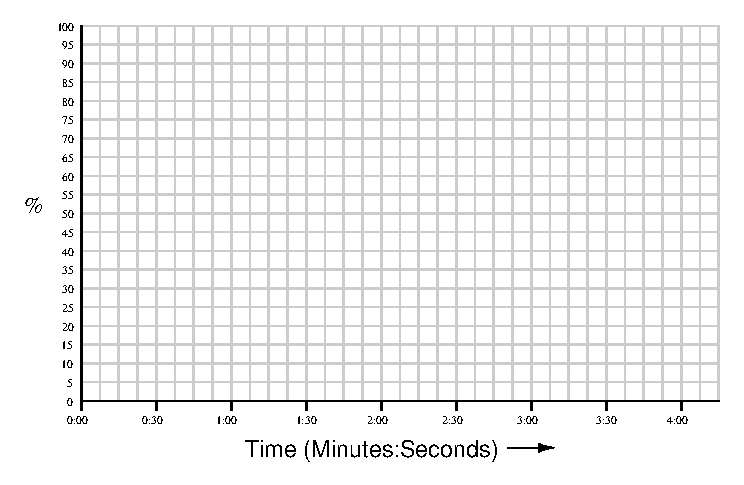
\includegraphics[width=13cm]{i00073x01.eps}$$

\vskip 10pt

\noindent
{\bf Prosess med dødtid:}

$$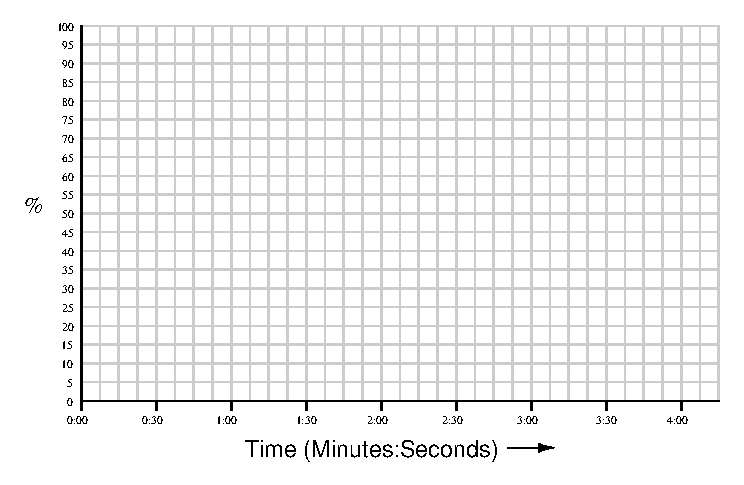
\includegraphics[width=13cm]{i00073x01.eps}$$


\underbar{file i00073no}
%(END_QUESTION)





%(BEGIN_ANSWER)

This is a graded question -- no answers or hints given!

%(END_ANSWER)





%(BEGIN_NOTES)


%INDEX% Control, PID tuning: process characterization

%(END_NOTES)
